\documentclass[a5paper]{article}
\usepackage{tikz}
\usepackage[margin=0.4cm]{geometry}
\usepackage{amsmath, amssymb, amsfonts}
\usepackage{graphicx}
\usepackage{enumitem}
\usepackage{multicol}
\usepackage{titlesec}
\usepackage{hyperref}

% Set up compact sections
\titlespacing*{\section}{0pt}{*2}{*1}
\titlespacing*{\subsection}{0pt}{*1.5}{*0.8}

\begin{document}

\title{Formularium Wiskunde}
\author{Ian Claesen}
\date{}
\maketitle

\tableofcontents

\section{Algebra}
\subsection{Volgorde van Bewerking}
Haakjes wegwerken, machtsverheffen, worteltrekken, vermenigvuldigen en delen, optellen en aftrekken. Om deze volgorde te onthouden, gebruik de ezelsbrug: \\ \textit{Heel Mooie Witte Vaatwassers Doen Onze Afwas}.

\subsection{Absolute Waarde}
De absolute waarde van een getal $a$ wordt genoteerd als $|a|$ en is altijd positief.
\[
|a| = \begin{cases} 
a & \text{if } a \geq 0 \\
-a & \text{if } a < 0 
\end{cases}\]

\newpage

\section{Machten en wortels}
\subsection{Machten met Gehele Exponenten}
\renewcommand{\arraystretch}{1.5} % Adjust row height

\[
\begin{array}{|c|c|}
\hline
\begin{array}{l}
\forall a \in ,\forall n \in {\mathbb{N}_0}:{a^n} = \underbrace {a.a.\;...\;.a}_{n\;factoren}\\
\forall a \in {\mathbb{R}}:\;{a^1} = \;a\\
\forall a \in {\mathbb{R}_0}:\;{a^0} = \;1\\
\forall a \in {\mathbb{R}_0},\forall n \in {\mathbb{N}}:\;{a^{ - n}} = \;\frac{1}{{{a^n}}}
\end{array} & \begin{array}{l}
\forall a,b \in {\mathbb{R}_0},\forall m,n \in {\mathbb{Z}}:{a^m} \cdot {a^n} = {a^{m + n}}\\
\frac{{{a^m}}}{{{a^n}}} = {a^{m - n}}\\
{({a^m})^n} = {a^{mn}}\\
{(a.b)^n} = {a^n} \cdot {b^n}\\
{\left( {\frac{a}{b}} \right)^n} = \frac{{{a^n}}}{{{b^n}}}\\
{\left( {\frac{a}{b}} \right)^{ - n}} = {\left( {\frac{b}{a}} \right)^n}
\end{array} \\ 
\hline
\end{array}
\]

\subsection{Vierkantswortel in $\mathbb{R}$}

\[
\begin{array}{|c|c|}
\hline
\begin{array}{l}
\forall a\in\mathbb{R}^+,\forall b\in\mathbb{R}:\\
 b=\sqrt a\Leftrightarrow b^2=a\,\land\,(b\geq0)\\
\forall a,b\in\mathbb{R}^+:\\
\hspace{1cm}\sqrt{a^2}=a\\
\hspace{1cm}\left(\sqrt a\right)^2=a\\
\hspace{1cm}\sqrt{ab} = \sqrt{a} \cdot \sqrt{b}.\\
\hspace{1cm}\sqrt{\frac{a}{b}} = \frac{\sqrt{a}}{\sqrt{b}} \land b \neq 0\\
\end{array} & \begin{array}{l}
\forall a\in\mathbb{R}:\\
\sqrt{a^2} = \left|a\right| \implies 
\begin{cases} 
    \sqrt{a^2} = a & \text{als } a \geq 0, \\ 
    \sqrt{a^2} = -a & \text{als } a \leq 0.
\end{cases}
\end{array} \\ 
\hline
\end{array}
\]

\subsection{N-de machtswortel in $\mathbb{R}$}
\[
\begin{array}{|c|c|}
\hline
\begin{array}{l}
n\,\,even\Rightarrow\sqrt[n]{a^n}=\left|a\right|\rightarrow\left\{\begin{matrix}\sqrt[n]{a^n}=a&\land\, a\geq0\\\sqrt[n]{a^n}=-a&\land\, a\le0\\\end{matrix}\right.\,\\
n\,\, oneven\Rightarrow\sqrt[n]{a^n}=a
\end{array} & \begin{array}{l}
\forall a,b\in\mathbb{R}_0^+,\forall m,n\in\mathbb{N}_0:\\
\sqrt[n]{a^n}=a\\
\left(\sqrt[n]{a}\right)^n=a\\
\sqrt[n]{ab}=\sqrt[n]{a}.\sqrt[n]{b}\\
\sqrt[n]{\frac{a}{b}}=\frac{\sqrt[n]{a}}{\sqrt[n]{b}}\\
\sqrt[m]{\sqrt[n]{a}}=\sqrt[m.n]{a}
\end{array} \\ 
\hline
\end{array}
\]
\subsection{$\frac{m}{n}$-de machtswortel in $\mathbb{R}$ }
\[
\begin{array}{|c|c|}
\hline
\begin{array}{l}
\forall a\in\mathbb{R}_0^+,\forall m\in\mathbb{Z},\forall n\in\mathbb{N}_0:a^\frac{m}{n}=\sqrt[n]{a^m}
\end{array} & \begin{array}{l}
\forall a,b\in\mathbb{R}_0^+,\forall m,n\in\mathbb{Q}:\\
a^m.a^n=a^{m+n}\\
\frac{a^m}{a^n}=a^{m-n}\\
\left(a^m\right)^n=a^{m.n}\\
\left(a.b\right)^m=a^m.b^m\\
\left(\frac{a}{b}\right)^m=\frac{a^m}{b^m}
\end{array} \\ 
\hline
\end{array}
\]
\newpage

\section{Veeltermen}
\subsection{Vierkantsvergelijking}
$Een\:vierkantsvergelijking\:is\:van\:de\:vorm:\:ax^2 + bx + c = 0\:,\:met\:D=b^2 - 4ac $

\renewcommand{\arraystretch}{1.5} % Adjust row height
\[
\begin{array}{|c|c|}
\hline
x\in{\displaystyle \mathbb {R} } & x\in{\displaystyle \mathbb {C} } \\ 
\hline
x_{1,2} = \frac{-b \pm \sqrt{D}}{2a} \quad  & x_{1,2} = \frac{-b \pm i\sqrt{-D}}{2a} \quad \\ 
\hline
P = \frac{c}{a} = x_1 \cdot x_2\:,\:S = -\frac{b}{a} = x_1 + x_2 &  \\ 
\hline
ax^2 + bx + c = a(x - x_1)(x - x_2) = a(x^2 - Sx + P) & \\
\hline
\end{array}
\]

\subsection{Merkwaardige Producten en Ontbinding in Factoren}
\[
\begin{array}{|l|l|}
\hline
(a\pm b)^2 = a^2 \pm 2ab + b^2 \\ 
\hline
{\left( {a \pm b} \right)^3} = {a^3} \pm 3{a^2}b + 3a{b^2} \pm {b^3} \\
\hline
{\left( {a + b} \right)^n} = {a^n} + C_n^1{a^{n - 1}}b + C_n^2{a^{n - 2}}{b^2} + ... + C_n^{n - 1}{a^2}{b^{n - 1}} + {b^n}\quad  \wedge \quad C_n^p = \frac{{n!}}{{\left( {n - p} \right)!p!}} \\
\hline
{a^2} - {b^2} = \left( {a + b} \right)\left( {a - b} \right) \\
\hline
{a^3} - {b^3} = \left( {a - b} \right)\left( {{a^2} + ab + {b^2}} \right) \\
\hline
{a^n} - {b^n} = \left( {a - b} \right)\left( {{a^{n - 1}} + {a^{n - 2}}b + {a^{n - 3}}{b^2} + ... + a{b^{n - 2}} + {b^{n - 1}}} \right) \\
\hline
\end{array}
\]

\subsection{Euclidische Deling}
Schema van Horner
\[
\frac{(3x^3-5x^2+10x-52)}{(x-2)}
\]

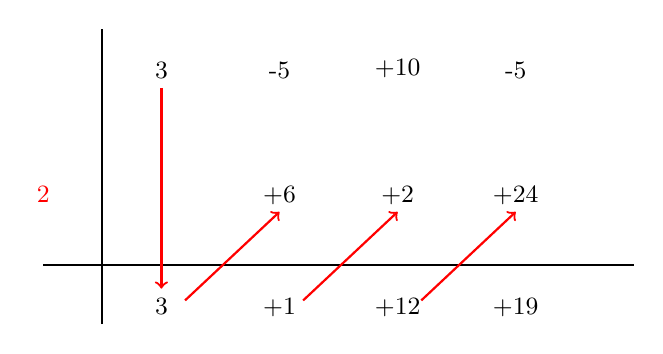
\begin{tikzpicture}[scale=1.5, every node/.style={font=\small}]
    % Draw the axes
    \draw[thick, -] (-0.5, 0) -- (4.5, 0); % Horizontal axis
    \draw[thick, -] (0, -0.5) -- (0, 2); % Vertical axis

    % Top row numbers
    \node[above] at (0.5, 1.5) {3};
    \node[above] at (1.5, 1.5) {-5};
    \node[above] at (2.5, 1.5) {+10};
    \node[above] at (3.5, 1.5) {-5};

    % Bottom row numbers
    \node[below] at (0.5, -0.2) {3};
    \node[below] at (1.5, -0.2) {+1};
    \node[below] at (2.5, -0.2) {+12};
    \node[below] at (3.5, -0.2) {+19};

    % Draw vertical arrow for the first step
    \draw[->, thick, red] (0.5, 1.5) -- (0.5, -0.2);
    \node[below,red] at (-0.5, 0.75) {$2$};

    % Draw horizontal arrows for the transformations
    \draw[->, thick, red] (0.7, -0.3) -- (1.5, 0.45);
    \node[below] at (1.5, 0.75) {+6};

    \draw[->, thick, red] (1.7, -0.3) -- (2.5, 0.45);
    \node[below] at (2.5, 0.75) {+2};

    \draw[->, thick, red] (2.7, -0.3) -- (3.5, 0.45);
    \node[below] at (3.5, 0.75) {+24};
\end{tikzpicture}

\newpage

\section{Complexe getallen}
\subsection{Rechthoekige coordinaten}
\[
\begin{array}{|l|l|}
\hline
\textbf{Bewerking} & \textbf{Formule} \\ \hline
Optelling/Aftrekking & (a + j.b) \pm (c + j.d) = (a + c) \pm j(b + d) \\ \hline
Vermenigvuldiging & (a + j.b) \cdot (c + j.d) = (ac - bd) + j(ad + bc) \\ \hline
Deling & 
\frac{(a + j.b)}{(c + j.d)} = \frac{(a + j.b) \cdot (c - j.d)}{(c + j.d) \cdot (c - j.d)} = \left( \frac{ac + bd}{c^2 + d^2} \right) + j \left( \frac{bc - ad}{c^2 + d^2} \right) \\ \hline
Toegevoegde\:van & \overline{(a + j.b)} = (a - j.b) \\
& \overline{Z_1 + Z_2} = \overline{Z_1} + \overline{Z_2}, \quad \overline{Z_1 \cdot Z_2} = \overline{Z_1} \cdot \overline{Z_2} \\ \hline
Inverse & z = a + bi \implies z^{-1} = \frac{a - bi}{a^2 + b^2} \\ \hline
Wortel & 
\sqrt{a} \; \wedge \; a < 0 \implies \sqrt{a} = \pm i\sqrt{-a} \\ 
& \sqrt{a + bi} = x + yi \iff (x + yi)^2 = a + bi \\ \hline
Macht & 
(a + bi)^0 = 1 \quad \forall n \in \mathbb{N}_0: \\
& (a + bi)^n = (a + bi) \cdot (a + bi) \cdots (a + bi) \\ \hline
Machten\:of\:i & i^1 = i, \quad i^2 = -1, \quad i^3 = -i, \quad i^4 = 1 \\ \hline
\end{array}
\]

\subsection{Poolcoördinaten}
\[z = a + i.b = r\left( {\cos (\varphi ) + i.\sin (\varphi )} \right) = r\angle \varphi ,\quad \tan (\varphi ) = \frac{b}{a},\quad r = \sqrt {{a^2} + {b^2}} \]
\[
\begin{array}{|l|l|}
\hline
\textbf{Bewerking} & \textbf{Formule} \\
\hline
Vermenigvuldiging & {z_1} \cdot {z_2} = {r_1} \cdot {r_2}\angle {\varphi _1} + {\varphi _2} \\
\hline
Deling & \frac{{{z_1}}}{{{z_2}}} = \frac{{{r_1}\angle {\varphi _1}}}{{{r_2}\angle {\varphi _2}}} = \frac{{{r_1}}}{{{r_2}}}\angle {\varphi _1} - {\varphi _2} \\
\hline
Inverse & {z^{ - 1}} = \frac{1}{r}\angle  - \varphi  \\ \hline
Macht & {z^n} = {r^n}\left[ {\cos \left( {n \cdot \varphi } \right) + i\sin \left( {n \cdot \varphi } \right)} \right]\quad n \in {\displaystyle \mathbb {N} }\\
\hline
Wortel & 
\sqrt {r(\cos \varphi  + i\sin \varphi )}  =  \pm \sqrt r \left( {\cos \frac{\varphi }{2} + i\sin \frac{\varphi }{2}} \right)\\
\hline
\multicolumn{2}{|c|}{\sqrt[n]{{r\left( {\cos \varphi  + i\sin \varphi } \right)}} = \sqrt[n]{r}\left( {\cos \frac{{\varphi  + k \cdot 2\pi }}{n} + i\sin \frac{{\varphi  + k \cdot 2\pi }}{n}} \right)\quad  \wedge \quad k = 0,1, \cdots ,n - 1} \\
\hline
 \end{array}
\]

\newpage

\newpage

\section{Goniometrie}
\subsection{De Goniometrische Cirkel}
\begin{figure}[h]
\centering
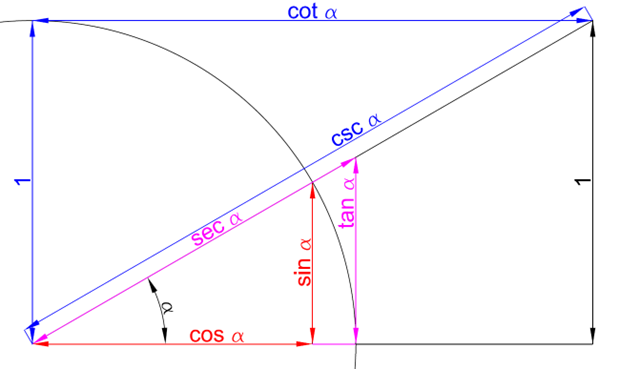
\includegraphics[width=0.8\textwidth]{imagegon.png}
\label{fig:voorbeeld}
\end{figure}

\subsection{formules uit de goniometrie}
\[
\begin{array}{|c|c|}
\hline
\begin{array}{c}
\csc \beta \quad \sec \beta \quad \cot \beta \\
\leftarrow \quad \leftarrow \quad \leftarrow \\
\textbf{os} \quad \textbf{as} \quad \textbf{oa} \\
\rightarrow \quad \rightarrow \quad \rightarrow \\
\sin \beta \quad \cos \beta \quad \tan \beta
\end{array}
& % Scheiding van de twee kolommen
\begin{array}{l}
\text{waarin:} 
\left\{
\begin{aligned}
& o: \text{ overstaande rechthoekszijde} \\
& s: \text{ schuine zijde (hypotenusa)} \\
& a: \text{ aanliggende rechthoekszijde}
\end{aligned}
\right.
\end{array} \\ 
\hline
\end{array}
\]

\[
\begin{array}{|c|c|}
\hline
\text{sin} \, \beta = \frac{b}{a} \hspace{1cm} \text{cos} \, \beta = \frac{c}{a} \hspace{1cm} \text{tan} \, \beta = \frac{b}{c} \hspace{1cm} \text{cot} \, \beta = \frac{c}{b} \hspace{1cm} \text{sec} \, \beta = \frac{a}{c} \hspace{1cm} \text{csc} \, \beta = \frac{a}{b} \\
\hline
\text{tan} \, \alpha = \frac{\sin \alpha}{\cos \alpha} \hspace{1cm} \text{cot} \, \alpha = \frac{\cos \alpha}{\sin \alpha} \hspace{1cm} \text{cot} \, \alpha = \frac{1}{\tan \alpha} \\
\hline
\text{sec} \, \alpha = \frac{1}{\cos \alpha} \hspace{1cm} \text{csc} \, \alpha = \frac{1}{\sin \alpha} \hspace{1cm} \\
\hline
\end{array}
\]


\[
\boxed{\sin^2{\alpha} + \cos^2{\alpha} = 1} \hspace{1cm}
\boxed{\tan^2{\alpha} + 1 = \sec^2{\alpha}} \hspace{1cm}
\boxed{1 + \cot^2{\alpha} = \csc^2{\alpha}}
\]
\newpage
\begin{figure}
    \centering
    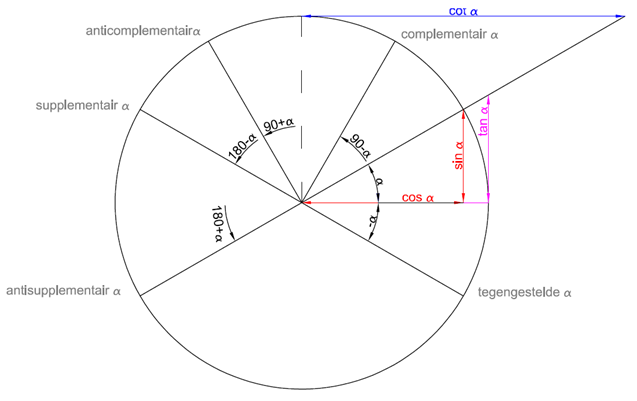
\includegraphics[width=1\linewidth]{imagfde.png}
  
    \label{fig:enter-label}
\end{figure}
\[
\begin{array}{|c|c|c|}
\hline
\text{gelijkehoeken} & \text{supplementairehoeken} & \text{complementairehoeken} \\
\hline
\sin{\left(\alpha + k2\pi\right)} = \sin{\alpha} & \sin{\left(\pi - \alpha\right)} = \sin{\alpha} & \sin{\left(\frac{\pi}{2} - \alpha\right)} = \cos{\alpha} \\
\cos{\left(\alpha + k2\pi\right)} = \cos{\alpha} & \cos{\left(\pi - \alpha\right)} = -\cos{\alpha} & \cos{\left(\frac{\pi}{2} - \alpha\right)} = \sin{\alpha} \\
\tan{\left(\alpha + k2\pi\right)} = \tan{\alpha} & \tan{\left(\pi - \alpha\right)} = -\tan{\alpha} & \tan{\left(\frac{\pi}{2} - \alpha\right)} = \cot{\alpha} \\
\cot{\left(\alpha + k2\pi\right)} = \cot{\alpha} & \cot{\left(\pi - \alpha\right)} = -\cot{\alpha} & \cot{\left(\frac{\pi}{2} - \alpha\right)} = \tan{\alpha} \\
\sec{\left(\alpha + k2\pi\right)} = \sec{\alpha} & \sec{\left(\pi - \alpha\right)} = -\sec{\alpha} & \sec{\left(\frac{\pi}{2} - \alpha\right)} = \csc{\alpha} \\
\csc{\left(\alpha + k2\pi\right)} = \csc{\alpha} & \csc{\left(\pi - \alpha\right)} = \csc{\alpha} & \csc{\left(\frac{\pi}{2} - \alpha\right)} = \sec{\alpha} \\
\hline
\end{array}
\]

\[
\begin{array}{|c|c|c|}
\hline
\text{tegengesteldehoeken} & \text{antisupplementairehoeken} & \text{anticomplementairehoeken} \\
\hline
\sin{\left(-\alpha\right)} = -\sin{\alpha} & \sin{\left(\pi + \alpha\right)} = -\sin{\alpha} & \sin{\left(\frac{\pi}{2} + \alpha\right)} = \cos{\alpha} \\
\cos{\left(-\alpha\right)} = \cos{\alpha} & \cos{\left(\pi + \alpha\right)} = -\cos{\alpha} & \cos{\left(\frac{\pi}{2} + \alpha\right)} = -\sin{\alpha} \\
\tan{\left(-\alpha\right)} = -\tan{\alpha} & \tan{\left(\pi + \alpha\right)} = \tan{\alpha} & \tan{\left(\frac{\pi}{2} + \alpha\right)} = -\cot{\alpha} \\
\cot{\left(-\alpha\right)} = -\cot{\alpha} & \cot{\left(\pi + \alpha\right)} = \cot{\alpha} & \cot{\left(\frac{\pi}{2} + \alpha\right)} = -\tan{\alpha} \\
\sec{\left(-\alpha\right)} = \sec{\alpha} & \sec{\left(\pi + \alpha\right)} = -\sec{\alpha} & \sec{\left(\frac{\pi}{2} + \alpha\right)} = -\csc{\alpha} \\
\csc{\left(-\alpha\right)} = -\csc{\alpha} & \csc{\left(\pi + \alpha\right)} = -\csc{\alpha} & \csc{\left(\frac{\pi}{2} + \alpha\right)} = \sec{\alpha} \\
\hline
\end{array}
\]

\newpage

\section{Meetkunde}
\subsection{De Cirkel}
De vergelijking van een cirkel met middelpunt $(a, b)$ en straal $r$ is:
\[
(x-a)^2 + (y-b)^2 = r^2
\]

\subsection{De Parabool}
De standaardvergelijking van een parabool met top in de oorsprong is:
\[
y = ax^2
\]

\section{Analyse}
\subsection{Limieten van Functies}
De limiet van een functie $f(x)$ als $x$ nadert tot $a$ wordt genoteerd als:
\[
\lim_{x \to a} f(x)
\]

\subsection{Afgeleiden}
De afgeleide van een functie $f(x)$ wordt gegeven door:
\[
f'(x) = \lim_{h \to 0} \frac{f(x+h) - f(x)}{h}
\]

\section{Matrices}
\subsection{Rekenregels}
Voor matrices $A$, $B$ en $C$ gelden de volgende eigenschappen:
\begin{itemize}
    \item Commutativiteit van optelling: $A + B = B + A$
    \item Associativiteit van optelling: $A + (B + C) = (A + B) + C$
    \item Distributiviteit: $A(B + C) = AB + AC$
\end{itemize}

\section{Combinatieleer}
\subsection{Keuzes zonder Herhaling}
\textbf{Variaties}: Geordende keuze van $p$ elementen uit $n$ elementen.\\
\textbf{Permutaties}: Het rangschikken van $n$ verschillende elementen.

\section{Kansrekening}
\subsection{Voorwaardelijke Kans}
De voorwaardelijke kans van $A$ gegeven $B$ is:
\[
P(A|B) = \frac{P(A \cap B)}{P(B)}
\]

\section{Statistiek}
\subsection{Normaalverdeling}
De normaalverdeling wordt gegeven door de dichtheidsfunctie:
\[
f(x) = \frac{1}{\sigma\sqrt{2\pi}} e^{-\frac{(x-\mu)^2}{2\sigma^2}}
\]

\section{Diversen}
\subsection{Wiskundige Symbolen}
\begin{itemize}
    \item $\in$: is een element van
    \item $\forall$: voor alle
    \item $\exists$: er bestaat
\end{itemize}

\end{document}
